\documentclass[letterpaper, 11pt]{article}
\pagestyle{plain}
\setlength{\textwidth}{7in}
\setlength{\oddsidemargin}{-0.1in}
\setlength{\evensidemargin}{-0.1in}
\setlength{\textheight}{9in}
\setlength{\topmargin}{0in}
\setlength{\headheight}{0in}
\setlength{\headsep}{0in}
\setlength{\footskip}{.5in}
\setlength {\parskip}{6pt}


\usepackage{amsmath}
\usepackage{amssymb}
\usepackage{amsthm}
\usepackage[linesnumbered,ruled]{algorithm2e}
\usepackage{todonotes}
\usepackage{enumitem}
\usepackage{times,amsxtra,latexsym,graphics,verbatim,epsfig,setspace,subfigure,epic}
\usepackage{xspace,prettyref}
\usepackage{bbm}
\usepackage{authblk}

\usepackage{tikz}
\usetikzlibrary{shapes,snakes}

\DeclareMathOperator*{\inv}{In}
\DeclareMathOperator*{\argmin}{argmin}
\DeclareMathOperator*{\argmax}{argmax}


\newtheorem{definition}{Definition}[section]
\newtheorem{theorem}{Theorem}[section]
\newtheorem{remark}[theorem]{Remark}
\newtheorem{proposition}[theorem]{Proposition}
\newtheorem{corollary}[theorem]{Corollary}
\newtheorem{claim}[theorem]{Claim}
\newtheorem{lemma}[theorem]{Lemma}

\newcommand{\diverge}{\to\infty}
\newcommand{\eqdistr}{{\stackrel{\rm (d)}{=}}}
\newcommand{\iiddistr}{{\stackrel{\text{\iid}}{\sim}}}
\newcommand{\ones}{\mathbf 1}
\newcommand{\zeros}{\mathbf 0}
\newcommand{\reals}{{\mathbb{R}}}
\newcommand{\integers}{{\mathbb{Z}}}
\newcommand{\naturals}{{\mathbb{N}}}
\newcommand{\rationals}{{\mathbb{Q}}}
\newcommand{\naturalsex}{\overline{\mathbb{N}}}
\newcommand{\symm}{{\mbox{\bf S}}}  \newcommand{\supp}{{\rm supp}}
\newcommand{\eexp}{{\rm e}}
\newcommand{\rexp}[1]{{\rm e}^{#1}}

\newcommand{\diff}{{\rm d}}
\newcommand{\red}{\color{red}}
\newcommand{\blue}{\color{blue}}
\newcommand{\nb}[1]{{\sf\blue[#1]}}
\newcommand{\nbr}[1]{{\sf\red[#1]}}
\newcommand{\Expect}{\mathbb{E}}
\newcommand{\expect}[1]{\mathbb{E}\left[ #1 \right]}
\newcommand{\expects}[2]{\mathbb{E}_{#2}\left[ #1 \right]}
\newcommand{\tExpect}{{\tilde{\mathbb{E}}}}
\newcommand{\Prob}[1]{{ \mathbb{P}\left\{ #1 \right\} }}
\newcommand{\tProb}{{\tilde{\mathbb{P}}}}
\newcommand{\tprob}[1]{{ \tProb\left\{ #1 \right\} }}
\newcommand{\hProb}{\widehat{\mathbb{P}}}
\newcommand{\toprob}{\xrightarrow{\Prob}}
\newcommand{\tolp}[1]{\xrightarrow{L^{#1}}}
\newcommand{\toas}{\xrightarrow{{\rm a.s.}}}
\newcommand{\toae}{\xrightarrow{{\rm a.e.}}}
\newcommand{\todistr}{\xrightarrow{{\rm D}}}
\newcommand{\toweak}{\rightharpoonup}
\newcommand{\var}{\mathsf{var}}
\newcommand{\Var}[1]{\mathbf{Var}\left[ #1 \right] }
\newcommand{\Cov}{\text{Cov}}
\newcommand\indep{\protect\mathpalette{\protect\independenT}{\perp}}
\def\independenT#1#2{\mathrel{\rlap{}\mkern2mu{#1#2}}}
\newcommand{\Bern}{{\rm Bern}}
\newcommand{\Binom}{{\rm Binom}}
\newcommand{\Pois}{{\rm Pois}}
\newcommand{\Hyp}{{\rm Hyp}}
\newcommand{\eg}{e.g.\xspace}
\newcommand{\ie}{i.e.\xspace}
\newcommand{\iid}{i.i.d.\xspace}
\newrefformat{eq}{(\ref{#1})}
\newrefformat{chap}{Chapter~\ref{#1}}
\newrefformat{sec}{Section~\ref{#1}}
\newrefformat{algo}{Algorithm~\ref{#1}}
\newrefformat{fig}{Fig.~\ref{#1}}
\newrefformat{tab}{Table~\ref{#1}}
\newrefformat{rmk}{Remark~\ref{#1}}
\newrefformat{clm}{Claim~\ref{#1}}
\newrefformat{def}{Definition~\ref{#1}}
\newrefformat{cor}{Corollary~\ref{#1}}
\newrefformat{lmm}{Lemma~\ref{#1}}
\newrefformat{prop}{Proposition~\ref{#1}}
\newrefformat{app}{Appendix~\ref{#1}}
\newrefformat{hyp}{Hypothesis~\ref{#1}}
\newrefformat{thm}{Theorem~\ref{#1}}
\newcommand{\ntok}[2]{{#1,\ldots,#2}}
\newcommand{\pth}[1]{\left( #1 \right)}
\newcommand{\qth}[1]{\left[ #1 \right]}
\newcommand{\sth}[1]{\left\{ #1 \right\}}
\newcommand{\bpth}[1]{\Bigg( #1 \Bigg)}
\newcommand{\bqth}[1]{\Bigg[ #1 \Bigg]}
\newcommand{\bsth}[1]{\Bigg\{ #1 \Bigg\}}
\newcommand{\norm}[1]{\left\|{#1} \right\|}
\newcommand{\lpnorm}[1]{\left\|{#1} \right\|_{p}}
\newcommand{\linf}[1]{\left\|{#1} \right\|_{\infty}}
\newcommand{\lnorm}[2]{\left\|{#1} \right\|_{{#2}}}
\newcommand{\Lploc}[1]{L^{#1}_{\rm loc}}
\newcommand{\hellinger}{d_{\rm H}}
\newcommand{\Fnorm}[1]{\lnorm{#1}{\rm F}}
\newcommand{\fnorm}[1]{\|#1\|_{\rm F}}
\newcommand{\opnorm}[1]{\left\| #1 \right\|_2}
\newcommand{\iprod}[2]{\left \langle #1, #2 \right\rangle}
\newcommand{\Iprod}[2]{\langle #1, #2 \rangle}
\newcommand{\indc}[1]{{\mathbf{1}_{\left\{{#1}\right\}}}}
\newcommand{\Indc}{\mathbf{1}}

\newcommand{\dTV}{d_{\rm TV}}
\newcommand{\tb}{\widetilde{b}}
\newcommand{\tr}{\widetilde{r}}
\newcommand{\tc}{\widetilde{c}}
\newcommand{\tu}{{\widetilde{u}}}
\newcommand{\tv}{{\widetilde{v}}}
\newcommand{\tx}{{\widetilde{x}}}
\newcommand{\ty}{{\widetilde{y}}}
\newcommand{\tz}{{\widetilde{z}}}
\newcommand{\tA}{{\widetilde{A}}}
\newcommand{\tB}{{\widetilde{B}}}
\newcommand{\tC}{{\widetilde{C}}}
\newcommand{\tD}{{\widetilde{D}}}
\newcommand{\tE}{{\widetilde{E}}}
\newcommand{\tF}{{\widetilde{F}}}
\newcommand{\tG}{{\widetilde{G}}}
\newcommand{\tH}{{\widetilde{H}}}
\newcommand{\tI}{{\widetilde{I}}}
\newcommand{\tJ}{{\widetilde{J}}}
\newcommand{\tK}{{\widetilde{K}}}
\newcommand{\tL}{{\widetilde{L}}}
\newcommand{\tM}{{\widetilde{M}}}
\newcommand{\tN}{{\widetilde{N}}}
\newcommand{\tO}{{\widetilde{O}}}
\newcommand{\tP}{{\widetilde{P}}}
\newcommand{\tQ}{{\widetilde{Q}}}
\newcommand{\tR}{{\widetilde{R}}}
\newcommand{\tS}{{\widetilde{S}}}
\newcommand{\tT}{{\widetilde{T}}}
\newcommand{\tU}{{\widetilde{U}}}
\newcommand{\tV}{{\widetilde{V}}}
\newcommand{\tW}{{\widetilde{W}}}
\newcommand{\tX}{{\widetilde{X}}}
\newcommand{\tY}{{\widetilde{Y}}}
\newcommand{\tZ}{{\widetilde{Z}}}


\newcommand{\sfa}{{\mathsf{a}}}
\newcommand{\sfb}{{\mathsf{b}}}
\newcommand{\sfc}{{\mathsf{c}}}
\newcommand{\sfd}{{\mathsf{d}}}
\newcommand{\sfe}{{\mathsf{e}}}
\newcommand{\sff}{{\mathsf{f}}}
\newcommand{\sfg}{{\mathsf{g}}}
\newcommand{\sfh}{{\mathsf{h}}}
\newcommand{\sfi}{{\mathsf{i}}}
\newcommand{\sfj}{{\mathsf{j}}}
\newcommand{\sfk}{{\mathsf{k}}}
\newcommand{\sfl}{{\mathsf{l}}}
\newcommand{\sfm}{{\mathsf{m}}}
\newcommand{\sfn}{{\mathsf{n}}}
\newcommand{\sfo}{{\mathsf{o}}}
\newcommand{\sfp}{{\mathsf{p}}}
\newcommand{\sfq}{{\mathsf{q}}}
\newcommand{\sfr}{{\mathsf{r}}}
\newcommand{\sfs}{{\mathsf{s}}}
\newcommand{\sft}{{\mathsf{t}}}
\newcommand{\sfu}{{\mathsf{u}}}
\newcommand{\sfv}{{\mathsf{v}}}
\newcommand{\sfw}{{\mathsf{w}}}
\newcommand{\sfx}{{\mathsf{x}}}
\newcommand{\sfy}{{\mathsf{y}}}
\newcommand{\sfz}{{\mathsf{z}}}
\newcommand{\sfA}{{\mathsf{A}}}
\newcommand{\sfB}{{\mathsf{B}}}
\newcommand{\sfC}{{\mathsf{C}}}
\newcommand{\sfD}{{\mathsf{D}}}
\newcommand{\sfE}{{\mathsf{E}}}
\newcommand{\sfF}{{\mathsf{F}}}
\newcommand{\sfG}{{\mathsf{G}}}
\newcommand{\sfH}{{\mathsf{H}}}
\newcommand{\sfI}{{\mathsf{I}}}
\newcommand{\sfJ}{{\mathsf{J}}}
\newcommand{\sfK}{{\mathsf{K}}}
\newcommand{\sfL}{{\mathsf{L}}}
\newcommand{\sfM}{{\mathsf{M}}}
\newcommand{\sfN}{{\mathsf{N}}}
\newcommand{\sfO}{{\mathsf{O}}}
\newcommand{\sfP}{{\mathsf{P}}}
\newcommand{\sfQ}{{\mathsf{Q}}}
\newcommand{\sfR}{{\mathsf{R}}}
\newcommand{\sfS}{{\mathsf{S}}}
\newcommand{\sfT}{{\mathsf{T}}}
\newcommand{\sfU}{{\mathsf{U}}}
\newcommand{\sfV}{{\mathsf{V}}}
\newcommand{\sfW}{{\mathsf{W}}}
\newcommand{\sfX}{{\mathsf{X}}}
\newcommand{\sfY}{{\mathsf{Y}}}
\newcommand{\sfZ}{{\mathsf{Z}}}


\newcommand{\calA}{{\mathcal{A}}}
\newcommand{\calB}{{\mathcal{B}}}
\newcommand{\calC}{{\mathcal{C}}}
\newcommand{\calD}{{\mathcal{D}}}
\newcommand{\calE}{{\mathcal{E}}}
\newcommand{\calF}{{\mathcal{F}}}
\newcommand{\calG}{{\mathcal{G}}}
\newcommand{\calH}{{\mathcal{H}}}
\newcommand{\calI}{{\mathcal{I}}}
\newcommand{\calJ}{{\mathcal{J}}}
\newcommand{\calK}{{\mathcal{K}}}
\newcommand{\calL}{{\mathcal{L}}}
\newcommand{\calM}{{\mathcal{M}}}
\newcommand{\calN}{{\mathcal{N}}}
\newcommand{\calO}{{\mathcal{O}}}
\newcommand{\calP}{{\mathcal{P}}}
\newcommand{\calQ}{{\mathcal{Q}}}
\newcommand{\calR}{{\mathcal{R}}}
\newcommand{\calS}{{\mathcal{S}}}
\newcommand{\calT}{{\mathcal{T}}}
\newcommand{\calU}{{\mathcal{U}}}
\newcommand{\calV}{{\mathcal{V}}}
\newcommand{\calW}{{\mathcal{W}}}
\newcommand{\calX}{{\mathcal{X}}}
\newcommand{\calY}{{\mathcal{Y}}}
\newcommand{\calZ}{{\mathcal{Z}}}

\newcommand{\comp}[1]{{#1^{\rm c}}}
\newcommand{\Leb}{{\rm Leb}}
\newcommand{\Th}{{\rm th}}
\newcommand{\deltaC}{\delta_{N_i^*[t]}}


\renewcommand{\listalgorithmcfname}{List of Algorithms}
\renewcommand{\algorithmcfname}{Algorithm}
\renewcommand{\algorithmcfname}{Protocol}


\title{Reaching Approximate Byzantine Consensus with Multi-hop Communication\thanks{This research is supported in part by National Science Foundation awards NSF 1329681.
Any opinions, findings, and conclusions or recommendations expressed here are those of the authors
and do not necessarily reflect the views of the funding agencies or the U.S. government.}
}


\author{Lili Su\thanks{Address: 459 Coordinated Science Lab MC 228, 1308 W. Main St.
Urbana Illinois 61801, USA. \\
Email: lilisu3@illinois.edu. \\
Tel.: +12178985405
}}
\author{Nitin Vaidya}
\affil{ Department of Electrical and Computer Engineering\\ University of Illinois at Urbana-Champaign}






\begin{document}
\date{~}

\maketitle



~
\begin{abstract}
We address the problem of reaching consensus in the presence of Byzantine faults. In particular, we are interested in investigating the impact of messages relay on the network connectivity for a correct iterative approximate Byzantine consensus algorithm to exist.
The network is modeled by a simple directed graph. We assume a node can send messages to another node that is up to  hops away via forwarding by the intermediate nodes on the routes,
where  is a natural number. We characterize the necessary and sufficient topological conditions on the network structure. The tight conditions we found are consistent with the tight conditions identified in \cite{Vaidya2012IABC} for , where only local communication is allowed, and are strictly weaker
for . Let  denote the length of a longest path in the given network.  For  and undirected graphs, our conditions hold if and only if   and the node-connectivity of the given graph is at least  , where  is the total number of nodes and  is the maximal number of Byzantine nodes; and for  and directed graphs, our conditions is equivalent to the tight condition found in \cite{Tseng2014}, wherein exact Byzantine consensus is considered.

Our sufficiency is shown by constructing a correct algorithm, wherein the trim function is constructed based on investigating a newly introduced minimal messages cover property.
The trim function proposed also works over multi-graphs.


\end{abstract}





\newpage
\section{Introduction}
\label{sec:intro}





 Reaching consensus resiliently in the presence of Byzantine faults has been studied extensively in distributed computing \cite{Lamport1982, Rabin1983, Ben-Or1983, AA_Fekete_aoptimal,Ben-Or2010}. Messages relay is the relaying of a message from its source toward its ultimate destination through intermediate nodes.
We say a messages relay is bounded if each source node can only reliably/noislessly send messages to a destination node that is up to  hops away, where , termed as relay depth. Our focus is on investigating the tradeoff between the relay depth  and the network connectivity for a correct iterative approximate Byzantine consensus algorithm to exist. Let  be the length of a longest path in the network. The two special cases,  and , respectively, have already been well studied.

Under the full forwarding model, i.e., , a node is able to reliably send messages to another node via every possible route in the network. Let  be the total number of nodes in the network, it has been shown that given  Byzantine nodes, if the network node-connectivity is at least  and , there exist algorithmic solutions for the fault-free nodes to reach consensus over all possible inputs. Conversely, if the network node-connectivity is strictly less than  or , then reaching consensus is not guaranteed \cite{impossible_proof_lynch}. Thus  node-connectivity and  are both necessary and sufficient.
However,  as a result of this communication assumption, the proposed algorithms require fault-free nodes to keep track of the \emph{entire} network topology, leading to huge consumption of both memory resource and computation power.
In contrast, iterative algorithms are typically characterized by local communication (among neighbors, or near-neighbors), simple computations performed repeatedly, and a small amount of state per node.
The purely local communication model (i.e., ), where a node can only send messages to its neighbors and no message forwarding is allowed, has also attracted extensive attention among researchers \cite{Benezit, leblanc_HiCoNs,jadbabaie_concensus,Vaidya2012IABC,Vaidyamatrix, vaidyaII}.
It has been shown that a correct iterative approximate Byzantine algorithm exists if and only if for any node partition  of a graph such that ,  and , either there exists a node  such that  or there exists a node  such that , where  is the collection of incoming neighbors of node .


 Our main contribution is to provide a family of tight sufficient and necessary conditions on the network topology for a correct iterative consensus algorithm to exist. Our sufficiency is proved by constructing a new simple iterative algorithm, whose trim function is based on investigating a newly introduced minimal messages cover property.
Our results bridge the existing aforementioned two streams of work, i.e., when  and , respectively, and fill the gap between these two models.






The rest of the paper is  organized as follows. Section \ref{sec: model} presents our models and the structure of iterative algorithms of interest. Our necessary condition is demonstrated in Section \ref{sec:necessary}, whose sufficiency is proved constructively in Section \ref{sec:sufficiency}. We shown in Section \ref{sec: extension} that our results are equivalent to the  node-connectivity and  conditions for undirected graph when . Section \ref{sec:conclusion} discusses possible relaxations of our fault model and concludes the paper.



\section{Problem setup and structure of iterative algorithms}
\label{sec: model}
\paragraph{Communication model}
The system is assumed to be {\em synchronous}.
The communication network is modeled as a simple {\em directed} graph . Define two functions  and  over a graph  as follows:   returns the set of  nodes, where , and  returns the set of directed edges between nodes in . Node  can send messages to node  if and only if there exists an --path of length at most  in , where  is a natural number.
In addition, we assume each node can send messages to itself as well, i.e.,  for all . For each node , let  be the set of nodes that can reach node  via at most  hops.
Similarly, denote the set of nodes that are reachable from node  via at most  hops by . Due to the existence of self-loops,  and . When , we write  and  as  and , respectively, for simplicity.
Note that node  may send a message to node  via different --paths. To capture this distinction in transmission routes, we represent a message as a tuple , where  and  indicates the path via which message  should be transmitted. Four functions are defined over . Let function  be  and let   be , whose images are the first entry and the second entry, respectively, of message . In addition, functions  and  are defined by   and  if   is an --path, i.e., message  is sent from node  to node .








\paragraph{Fault model}
Let  be the collection of faulty nodes in the system. We consider the Byzantine fault model with up to  nodes becoming faulty, i.e., .  A faulty node may {\em misbehave} arbitrarily. Possible misbehavior includes sending incorrect and mismatching (or inconsistent) messages to different neighbors. In addition, a faulty node  may tamper message  if it is in the transmission path, i.e., \footnote{Recall that  is the vertex set of a given graph and  denotes the collection of vertices along the route of message , including the source and the

  destination.}.
However, faulty nodes are only able to tamper , leaving  unchanged. This assumption is placed for ease of exposition, later in Section \ref{sec:conclusion} we relax this assumption by considering the possibilities that faulty nodes may also tamper messages paths or even fake and transmit non-existing messages.
Faulty nodes are also assumed to have complete knowledge of the execution of the algorithm, including the states of all nodes,
contents of messages the other nodes send to each other, and
the algorithm specification, so that they may potentially collaborate with each other adaptively.



\paragraph{Iterative approximate Byzantine consensus (IABC) algorithms}
\label{sec:iabc}

The iterative algorithms considered in this paper should have the following structure:
Each node  maintains state , with  denoting the state
of node  at the {\em end}\, of the -th iteration of the algorithm.
Initial state of node ,
, is equal to the initial {\em input}\, provided to node .
At the {\em start} of the -th iteration (), the state of
node  is .
The IABC algorithms of interest will require each node 
to perform the following three steps in iteration , where .
Note that the faulty nodes may deviate from this specification.

\begin{enumerate}
\item {\em Transmit step:} Transmit messages of the form  to nodes in , i.e., the nodes that are reachable from node  via at most  hops. If node  is an intermediate node on the route of some message, then node  forwards that message as instructed by the message path.
\item {\em Receive step:} Receive messages from , i.e., the nodes that can reach node  via at most  hops.
Denote by  the set of messages that node  received
at iteration . \item \textit{Update step:} Node  updates its state using a transition function , where  is a part of the specification of the algorithm, and takes as input the set .
\end{enumerate}
Note that at the --th iteration, between step two and step three, by sending message to itself node  is able to memorize its state in the immediate preceding iteration, i.e,. . However, at the end of update step, except for its updated state , no other information collected in current iteration or any of the previous iteration will be kept by node . In step three, in general,  is some trim function over the received messages collection . The trimming strategy may depends on message values, message routes, or both. In addition, different nodes are allowed to have different trimming strategies.

Let  be the largest state among the fault-free nodes at the end of the -th iteration, i.e., .
Since the initial state of each node is equal to its input,
 is equal to the maximum value of the initial input at the fault-free nodes. Similarly, we define  to be the smallest state at the --th iteration and  to be the smallest initial input.
For an IABC algorithm to be correct, the following two conditions must be satisfied:
\begin{itemize}
\item {\em Validity:} 

\item {\em Convergence:} 
\end{itemize}


Our focus is to identify the necessary and sufficient
conditions for the existence of a {\em correct} IABC algorithm (i.e.,
an algorithm satisfying the above validity and convergence conditions)
for a given  and a given .






\section{Necessary Conditions}
\label{sec:necessary}

For a correct IABC algorithm to exist, the underlying network  must satisfy the conditions presented in this section. A couple of definitions are needed before we are able to formally state our necessary conditions.

\begin{definition}
Let  be a set of vertices in  and  be a vertex in  such that . A --path is a path from some vertex  to vertex . A set  of vertices such that  is a --\emph{vertex cut} if every --path contains a vertex in . The minimum size of a --vertex cut is called the --connectivity and is denoted by . Similarly, a set  of vertices is an --\emph{restricted vertex cut} if the deletion of  destroys all --paths of length at most . Let  be the minimum size of such restricted vertex cut in .
\end{definition}
The first part of the above definition is the classical definition of node connectivity in graph theory. However, this definition is a global notion. In our communication model, we implicitly assume that each fault-free node only knows the local network topology up to its --th neighborhood. We adapt node connectivity to our model by restricting the length of the paths under consideration. Note that  for all , and that a --restricted vertex cut of  is the number of node 's incoming neighbors in , i.e., .



\begin{definition}
For non-empty disjoint sets of nodes  and  in , we say
  if and only if
 there exists a node  such that ;
 otherwise.
\end{definition}

Let  be a set of vertices in , denote the induced subgraph\footnote{An induced subgraph of , induced by vertex set , is the subgraph  with vertex set  such that . Recall that  and  are the vertex set and edge set, respectively, of a given graph.} of  induced by vertex set  by . We describe the necessary and sufficient condition below, whose necessity is proved in Theorem \ref{thm:nc} and sufficiency is shown constructively in Section \ref{sec:sufficiency}. For ease of future reference, we termed the condition as \emph{Condition NC}.

\noindent\textbf{Condition NC}:
For any node partition  of  such that  and , in the induced subgraph ,
at least one of the two conditions below must be true: (i) ; (ii) . 

Intuitively, Condition NC requires that either the set of nodes in  are able to collectively influence the state of a node in  or vice versa. Note that when , Condition NC becomes\\
\emph{``
For any node partition  of  such that  and , in the induced subgraph ,
at least one of the two conditions below must be true: (i) there exists a node  such that ; (ii) there exists a node  such that ."}, which is shown to be both necessary and sufficient without message relay in \cite{Vaidya2012IABC}.



\begin{theorem}
\label{thm:nc}
Suppose that a correct IABC algorithm exists for . Then  satisfies Condition NC.
\end{theorem}
We prove this theorem in Appendix \ref{app:necessary}. Our proof shares the same proof structure of Theorem 1 in \cite{Vaidya2012IABC}.
The basic idea is as follows: Suppose there exists a correct IABC algorithm, then we are able to find a node partition satisfying the conditions as listed in Condition NC,
such that under some Byzantine layout, and for some specific initial inputs, convergence condition will be violated.






The above necessary condition is in general stronger than the necessary condition derived under single-hop message transmission model (i.e., ) \cite{Vaidya2012IABC}.
Consider the system depicted in Fig. \ref{example}.  The topology of this system does not satisfy the necessary condition derived in \cite{Vaidya2012IABC}. Since in the node partition  and , neither  nor  holds for . However, via enumeration it can be seen that the above graph (depicted in Fig. \ref{example}) satisfies Condition NC when . Nevertheless, increasing relay depth does not always admit more graph structures. For instance, for ,  and any , the only graph that satisfy Condition NC is the complete graph.

It follows from the definition of Condition NC that if a graph  satisfies Condition NC for , then  also satisfies Condition NC for all . Let  be the smallest integer for which  satisfies Condition NC, where  by convention if  does not satisfy Condition NC for any . We observe that in general given a graph , the diameter of  can be arbitrarily smaller than . For instance, the diameter of the graph depicted in Fig. \ref{example2} is two. However, for the depicted graph,  when  is odd. So  is much larger than two for large .

 \begin{figure}

 \centering
    \scalebox{1.2}{

    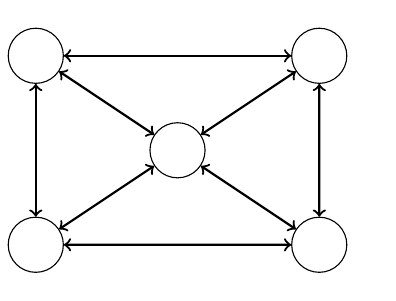
\begin{tikzpicture}[auto, scale=1.2]

\node[draw,circle,minimum size=0.7cm,inner sep=0pt] (A) at (0,0)  { };
     \node [draw,circle,minimum size=0.7cm,inner sep=0pt] (D) at (0,-2) {};
      \node [draw,circle,minimum size=0.7cm,inner sep=0pt] (B) at (3,0) {};
       \node [draw,circle,minimum size=0.7cm,inner sep=0pt] (C) at (3,-2) {};
       \node [draw,circle,minimum size=0.7cm,inner sep=0pt] (E) at (1.5,-1) {};

      \draw[<->, thick] (A)--(B);
      \draw[<->, thick] (B) -- (C);
      \draw[<->, thick] (D) -- (C);
      \draw[<->, thick] (A) -- (D);

      \draw[<->, thick] (A) -- (E);
      \draw[<->, thick] (B) -- (E);
      \draw[<->, thick] (C) -- (E);
      \draw[<->, thick] (D) -- (E);
    \end{tikzpicture}
    }
    \caption{In this system, there are five processors  and ; all communication links are bi-directional; and at most one processor can be adversarial, i.e., . }
    \label{example}
    \end{figure}




\begin{figure}

 \centering
    \scalebox{1.2}{

    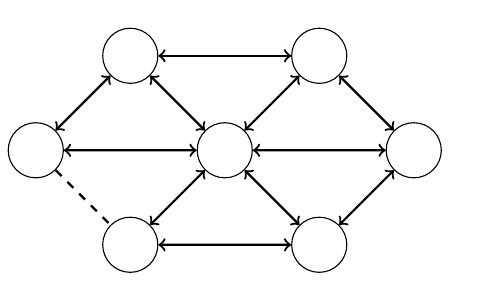
\begin{tikzpicture}[auto, scale=1.2]

\node[draw,circle,minimum size=0.7cm,inner sep=0pt] (A) at (0,0)  { };
     \node [draw,circle,minimum size=0.7cm,inner sep=0pt] (B) at (-1,-1) {};
     \node [draw,circle,minimum size=0.7cm,inner sep=0pt] (C) at (0,-2) {};

      \node [draw,circle,minimum size=0.7cm,inner sep=0pt] (D) at (2,-2) {};
       \node [draw,circle,minimum size=0.7cm,inner sep=0pt] (E) at (3,-1) {};
        \node[draw,circle,minimum size=0.7cm,inner sep=0pt] (F) at (2,0)  { };
\node [draw,circle,minimum size=0.7cm,inner sep=0pt] (G) at (1,-1) {};
      \draw[<->, thick] (A)--(B);
      \draw[-, dashed, thick] (B) -- (C);
      \draw[<->, thick] (D) -- (C);
      \draw[<->, thick] (D) -- (E);
      \draw[<->, thick] (E) -- (F);
      \draw[<->, thick] (F) -- (A);
      \draw[<->, thick] (A) -- (G);
      \draw[<->, thick] (B) -- (G);
      \draw[<->, thick] (C) -- (G);
      \draw[<->, thick] (D) -- (G);
      \draw[<->, thick] (E) -- (G);
      \draw[<->, thick] (F) -- (G);
    \end{tikzpicture}
    }
    \caption{In this system, there are  processors ; all communication links are bi-directional; and at most one processor can be adversarial, i.e., . Nodes  form a cycle of length  and these nodes are all connected to node . }
    \label{example2}
    \end{figure}


Similar to \cite{Vaidya2012IABC}, as stated in our next corollary, our Condition NC for general  also implies a lower bound on both the graph size  and the incoming degree of each node. Moreover, this lower bound is independent of .
\begin{corollary}
\label{cdegree}
If  satisfies Condition NC, then
  must be at least , and each node must have at least  incoming neighbors other than itself, i.e., .
\end{corollary}
The proof of Corollary \ref{cdegree} can be found in Appendix \ref{app:cdegree}. Note that Corollary \ref{cdegree} also characterizes a lower bound on the density of , that is , including self-loops, which is independent of the relay depth  as well. Proposition \ref{density} says that for , communication over multi-hop does not imply the existence of a sparser graph for which Condition NC holds than that with communication over single-hop. For  whether there exists a graph satisfying Condition NC with  and  edges or not for any  is still open.


\begin{proposition}
\label{density}
For  and , there exists a graph  for any  such that
(i)  for all ; and
(ii) .
\end{proposition}






\subsection{Equivalent Characterization of Condition NC}
Informally speaking, Condition NC describes the information propagation property in terms of four sets partitions. In this subsection, an equivalent condition of Condition NC is proposed, which is based on characterizing the structure of the special subgraphs, termed as reduced graph, of the power graph . The new condition suggests that all fault-free nodes will be influence by a collection of common fault-free nodes.

\begin{definition}
\label{def:decompose}
{\bf Meta-graph of SCCs:}
Let  be the strongly connected components (i.e., SCCs) of . The graph of SCCs, denoted by , is defined by\\
(i) Nodes are ; and\\
(ii) there is an edge  if there is some  and  such that  is an edge in .\\
Strongly connected component  is said to be a {\em source component}
if the corresponding node in  is \underline{not} reachable from any
other node in .
\end{definition}
It is known that the  is a directed acyclic graph ( i.e., DAG ) \cite{dag_decomposition}, which contains no directed cycles. It can be easily checked that due to the absence of directed cycles and finiteness, there exists one node in  that is not reachable from any other node. That is, a graph  has at least one source component.
\begin{definition}
The --th power of a graph , denoted by ,  is a graph with the same set of vertices as  and a directed edge between two vertices  if and only if there is a path of length  from  to  in .
\end{definition}

A path of length one between vertices  and  in  exists if  is an edge in . And a path of length two between vertices  and  in  exists for every vertex  such that  and  are edges in .
Then for a given graph  with self-loop at each node,
the  element in the square of the adjacency matrix of  counts the number of paths of length at most two in . Similarly, the  element in the --th power of the adjacency matrix of  gives the number of paths of length at most  between vertices  and  in .
The power graph  is a multigraph\footnote{A multigraph (or pseudograph) is a graph which is permitted to have multiple edges between each vertex pair, that is, edges that have the same end nodes. Thus two vertices may be connected by more than one edge.} and there is a one-to-one correspondence between an edge  in  and a path of length at most  in . Let  be an edge in , and let  be the corresponding path in , we say an edge  in  is covered by node set , if , i.e., path  passes through a node in .



\begin{definition}[Reduced Graph]
\label{def:reduced} 

For a given graph  and , let  be the set of edges in  that are covered by node set . For each node , choose  such that . Let  be the set of incoming edges of node  in  that are covered by node set .
  A reduced graph of , denoted by , is a subgraph of  whose node set and edge set are defined by (i)~ ; and
(ii) , respectively.
\end{definition}

Note that for a given  and a given ,
multiple reduced graphs may exist.
Let us define set  to be the collection of all reduced graph of  for a given , i.e.,



Since , the --th power of the induced subgraph , itself is a reduced graph of , where we choose  for each , thus  is nonempty.
 In addition,  is finite since the graph  is finite,


\begin{theorem}
\label{thm:nc2}
Graph  satisfies Condition NC if and only if every reduced graph  obtained as per Definition \ref{def:reduced}
must contain exactly one {\em source component}.
\end{theorem}


\section{Sufficiency: Algorithm 1}
\label{sec:sufficiency}

As aforementioned, for each node , the collection of received messages  may contains bogus messages and/or tampered messages due to the existence of Byzantine nodes, thus  is in general a trimming function. In this section we propose an algorithm, termed Algorithm 1, using a novel update/trimming strategy and show its correctness. First we introduce the definition of message cover that will be used frequently in this section. 











\begin{definition}

  For a communication graph , let  be a set of messages, and let  be the set of paths corresponding to all the messages in , i.e., . A message cover of  is a set of nodes , such that for each path , we have . In particular, a minimum message cover is defined by


 Conversely, given a set of messages  and a set of nodes , a maximal set of messages  that are covered by  is defined by,
 
\end{definition}

We further need the following two definitions before we are able to proceed to the description of our algorithm. Recall that  is the collection of messages received by node  at iteration . Let 
Sort messages in  in an increasing order, according to their message values, i.e.,  for .
Let  such that
(i) for all  and  we have ;
and (ii) the cardinality of a minimum cover of  is exactly , i.e., .
Similarly, we define  as follows:
(i) for all  and  we have ;
and (ii) the cardinality of a minimum cover of  is exactly , i.e., .
In addition, define .

\begin{theorem}
\label{trimming}
Suppose that graph  satisfies Condition NC, then the sets of messages ,  are well-defined and   is nonempty.
\end{theorem}
This theorem is proved by construction, i.e., an algorithm is constructed to find the sets ,  for a given . Details of the algorithm and its correctness proof can be found in Appendix \ref{trimmingProof}. With this trimming strategy at hand, 
we will prove that there exists an IABC algorithm -- particularly
{\em Algorithm 1} below -- that satisfies
the {\em validity} and {\em convergence} conditions provided that the
graph  satisfies Condition NC. This implies that Condition NC is also sufficient. {\em Algorithm 1} has the three-step structure described
in Section~\ref{sec:iabc}.







\vspace*{8pt}\hrule
{\,

\bf Algorithm 1}
\vspace*{4pt}\hrule

\begin{enumerate}
\label{algorithm}
\item {\em Transmit step:} Transmit messages of the form  to nodes in . If node  is an intermediate node of some message, then node  forwards that message as instructed by the message path.
    When node  expects to receive a message from a path but does not receive the message, the message value is assumed to be equal to some default message.

\item {\em Receive step:} Receive messages from .


\item {\em Update step:}


Define

where .


\end{enumerate}
\hrule
\,

Recall .
The ``weight'' of each term on the right-hand side of (\ref{e_Z}) is , where , and these weights add to 1.
For future reference, let us define , which is used in Theorem \ref{claim_1}, as:

In \emph {Algorithm 1}, each fault-free node 's state, ,  is updated as a convex combination of all the \emph{messages values} collected by node  at round . In particular, for each message , its coefficient is  if the message is in  or the message is sent via self-loop of node ; otherwise, the coefficient of  is zero.
The update step in \emph {Algorithm 1} is a generalization of the update steps proposed in \cite{Vaidyamatrix,IBA_broadcast_Sundaram}, where the update summation is over all the incoming neighbors of node  instead of over message routes. In \cite{Vaidyamatrix,IBA_broadcast_Sundaram}, only single-hop communication is allowed, i.e., , and the fault-free node  can receive only one message from its incoming neighbor. With multi-hop communication, fault-free node can possibly receive messages from a node via multiple routes. Our trim functions in \emph {Algorithm 1} take the possible multi-route messages into account. In fact, \emph {Algorithm 1} also works with multi-graphs.







\subsection{Matrix Representation of Algorithm 1}
\label{s_claim}

With our trimming function, the iterative update of the state
of a fault-free node  admits a nice matrix representation of states evolution of fault-free nodes.  We use boldface upper case letters to denote matrices, rows of matrices, and their entries. For instance,  denotes a matrix,  denotes the -th row of matrix , and  denotes the element at the intersection of the -th row and the -th column of matrix . Some useful concepts and theorems are reviewed briefly in Appendix \ref{MatrixPreliminaries}.

\begin{definition}
\label{d_stochastic}
A vector is said to be {\em stochastic} if all the entries
of the vector are {\em non-negative}, and the entries add up to 1.
A matrix is said to be row stochastic if each row of the matrix is a
stochastic vector.
\end{definition}

Recall that  is the set of faulty nodes and .
Without loss of generality, suppose that nodes 1 through  are
fault-free, and if , nodes  through  are faulty.
Denote by  the column vector consisting of the initial states of
all the {\em fault-free} nodes.
Denote by , where , the column vector consisting of
the states of all the {\em fault-free} nodes
at the end of the -th iteration, , where the -th element
of vector  is state . \begin{theorem}
\label{claim_1}
{
We can express the iterative update of the state
of a fault-free node  
performed in (\ref{e_Z}) using the matrix form in (\ref{e_matrix_i})
below,
where  satisfies the four conditions listed below.
In addition to , the row vector 
may depend on the state vector  as well as the
behavior of the faulty
nodes in . For simplicity, the notation  does not
explicitly represent this dependence.

}
\begin{enumerate}
\item  is a {\em stochastic} row vector of size .
Thus,
, where , and


\item .

\item  is non-zero
only if~~there exists a message  such that  and .
\item For any , there exists a reduced graph  with adjacent matrix  such that
, where  is some constant  to be specified in Claim \ref{claimw}.


\end{enumerate}
\end{theorem}
In Appendix \ref{app:claim_1}, we prove the correctness of Theorem \ref{claim_1} by constructing 
for . Our proof follows the same line of analysis as in the proof of Claim 2 in \cite{Vaidyamatrix}. Due to the complexity (in particular, the dependency of message covers) brought up by messages relay, we divide the universe into six cases to consider.



\begin{theorem}
\label{t}
\emph {Algorithm 1} satisfies the validity and the convergence conditions.
\end{theorem}



From the code of \emph {Algorithm 1}, we know that , where . Theorem \ref{claim_1} says that we can rewrite  as

where s together satisfy the preceding four conditions. By ``stacking'' (\ref{e_matrix_i}) for different
, , we can
represent the state update for all the fault-free nodes together
using (\ref{e_matrix})
below, where  is a  row stochastic matrix, with its -th row
being equal to  in (\ref{e_matrix_i}).

By repeated application of (\ref{e_matrix}), we obtain:

As the backward product  is a row-stochastic matrix, it holds that  for all  and all . Thus Algorithm 1 satisfies validity condition.

The convergence of  depends on the convergence of the backward product . As a result of this, our convergence proof uses toolkit of weak-ergodic theory that is also adopted in prior work
(e.g., \cite{Jadbabaie2003,Benezit,vaidyaII,leblanc_HiCoNs}),
with some similarities to the arguments used in \cite{vaidyaII,leblanc_HiCoNs}. The last condition in Theorem \ref{claim_1} plays an important role in the proof. For completeness, we present the formal proof of Theorem \ref{t} in Appendix \ref{app:correctness}.











\section{Connection with existing work under unbounded path length}
In this section, we show that Condition NC is equivalent to the existing results on both undirected graphs and directed graphs.  

\subsection{Undirected graph under unbounded path length}
\label{sec: extension}
If  is undirected, it has been shown in \cite{impossible_proof_lynch}, that  and node-connectivity  are both necessary and sufficient for achieving Byzantine approximate consensus. We will show that when , our Condition NC is equivalent to the above conditions.

\begin{theorem}
\label{equiUndirected}
  When , if  undirected, then  and the   node-connectivity of  is at least  if and only if  satisfies Condition NC.
\end{theorem}
Informally, if the node-connectivity of , denoted by , is at most , then we are able to show that there exists a node partition , where  are both nonempty and , such that neither  nor  holds. Conversely, if  and , using Expansion Lemma we are able to show Condition NC holds. Formal proof is given in Appendix \ref{app:connection}. 

\subsection{Directed graph under unbounded path length}

Synchronous exact Byzantine consensus is considered in \cite{Tseng2014}.  
\begin{definition}[\cite{Tseng2014}]
Given disjoint subsets , where  is non-empty: \\
(i) We say  if and only if set  contains at least  distinct incoming neighbors of . That is, .\\
(ii) We say  iff  is not true.
\end{definition}
A tight condition (both necessary and sufficient) over the graph structure is found in \cite{Tseng2014}.

\begin{theorem}[\cite{Tseng2014}]
Given a graph , exact Byzantine consensus is solvable if and only if for any partition  of , such that both  and  are non-empty, and , either , or .
\end{theorem}

We term this condition as Condition 1. Note that in order for  to hold, we only require that there are at least  incoming neighbors of set  in set . It is possible that each node in  has at most  incoming neighbors in . As a result of this observation, our Condition NC with  is strictly stronger than Condition 1. However, it can be shown that our Condition NC with  is equivalent to Condition 1. 

\begin{theorem}
\label{equivaDirected}
Condition NC is equivalent to Condition 1 when .
\end{theorem}

An alternative condition is shown in \cite{Tseng2014} to be equivalent to Condition 1. We use this condition as a bridging to show the equivalence of Condition 1 and Condition NC.

\section{Discussion and Conclusion}
\label{sec:conclusion}

Throughout this paper, we assume that faulty nodes are only able to tamper message values, leaving
message paths unchanged. However, even when faulty nodes are able to tamper message paths or even fake and transmit non-existing messages,
as long as (i) the number of faked messages is finite (each faulty node  cannot create too many non-existing messages);
and (ii) for each message  tampered/faked by the faulty node ,   must satisfy , i.e., the faulty node  cannot conceal itself from the message path,
using the same line of arguments as in Section \ref{sec:necessary} and Section \ref{sec:sufficiency}, it can be shown that the Condition NC is also necessary and sufficient for the existence of approximate consensus under the relaxed model.

In this paper, we unify two streams of work by assuming that each node knows the topology of up to its --th neighborhood and can send message to nodes that are up to  hops away, where . We prove a family of necessary and sufficient conditions for the existence
of {\em iterative}\, algorithms that achieve {\em approximate Byzantine consensus}
in arbitrary directed graphs.
The class of iterative algorithms considered in this paper ensures
that, after each iteration of the algorithm, the state of each fault-free node remains
in the {\em convex hull} of the states of the fault-free nodes at the end of
the previous iteration. 






\bibliographystyle{plain}
\bibliography{IBA}



\newpage
\appendix

\setlength {\parskip}{6pt}

\centerline{\Large\bf Appendices}
\section{Necessity of Condition NC}\label{app:necessary}


\begin{proof}[Proof of Theorem \ref{thm:nc}]
Theorem \ref{thm:nc} states that if a correct IABC algorithm exists for ,  then  satisfies:
For any node partition  of  such that  and , in the induced subgraph ,
at least one of the two conditions below must be true: (i) ; (ii) .

We prove this theorem by contradiction. Let us assume that a correct IABC exists, and there exists a partition  of  such that  and , but neither  nor  holds, i.e.,   and . Consider the case when all nodes in , if , are faulty, and the other nodes in sets  are fault-free. Note that the fault-free nodes are not aware of the identities of the faulty nodes. In addition, assume (i) each node in  has initial input , (ii) each node in  has initial input , such that  for some given constant , and (iii) each node in , if , has initial input in the interval .

In the \textit{Transmit step} of iteration one, suppose that each faulty node  sends  to nodes in , sends  to nodes in , and sends some arbitrary value in the interval  to nodes in . For message  such that the faulty node  is in its transmission path, i.e.,
, if , node  resets ; if , node  resets ; if
, node  resets  to be some arbitrary value in .

Consider any node .
Since , we know .
In addition,   holds in  implies . Let  be a minimum restricted --cut in .
From the perspective of node , there exist two possible cases:

\begin{enumerate}[label=\emph{(\alph*)}]
\item Both  and  are non-empty: We know  and .  From node 's perspective, two scenarios are possible: (1) nodes in  are faulty, all the messages relayed via them are tampered and the other nodes are fault-free, and (2) nodes in  are faulty and the other nodes are fault-free.

In scenario (1), from node 's perspective, the untampered values are in the interval . By validity condition, . On the other hand, in scenario (2), the untampered values are  and , where ; so , according to validity condition. Since node  does not know whether the correct scenario is (1) or (2), it must update its state to satisfy the validity condition in both cases. Thus, it follows that .

\item At most one of  and  is non-empty: Thus, . From node 's perspective, it is possible that the nodes in  are all faulty, the messages relayed via nodes in  are tampered while the rest of the nodes are fault-free. In this situation, the untampered values received by node  (which are all from nodes in ) are all , and therefore,  must be set to  as per the validity condition.
\end{enumerate}

At the end of iteration 1: for each node  in  ; similarly, for each node  in , ; if , for each node  in , . All these conditions are identical to the condition when . Then by a repeated application of of above argument, it follows that for any ,  for all ,  for all  and  for all , if .

Since  and  both contain fault-free nodes, the convergence requirement is not satisfied. This contradicts the assumption that a correct iterative algorithm exists.
\end{proof}

\subsection{Lower bound on graph size and nodes' incoming degrees} \label{app:cdegree}

\begin{proof}[Proof of Corollary \ref{cdegree}]
Corollary \ref{cdegree} states that if  satisfies Condition NC, then
  must be at least , and each node must have at least  incoming neighbors other than itself, i.e., .


The main
techniques used in this proof are fairly routine, and are given here
largely for both concreteness and completeness.

We first show the claim that .
For ,  is trivially true. For , the proof is by contradiction. Suppose that . In this case, we can partition  into sets  such that , ,  and , i.e.,  is empty. Since  and , we have  and , respectively in . This contradicts the assumption that  satisfies Condition NC. Thus, .

It remains to show .
Suppose that, contrary to our claim, there exists a node  such that .
Define set  and partition  into two sets  and 
such that 
and . Note that  if and only if .
Define  and . Since ,  is non-empty. From the construction of , we have , and .
Since ,  and , it follows that .
On the other hand, as , we have . This violates the assumption that  satisfies Condition NC. The proof is complete.
\end{proof}

\subsection{Lower bound on graph density}
\begin{proof}[Proof of Proposition \ref{density}]
Proposition \ref{density} states that: For  and , there exists a graph  for any  such that
(i)  for all ; and
(ii) .

We prove this proposition by inducting on .
In the complete graph with ,  ( including  itself ) for all  and the total number of edges is . So the base case easily follows. Assume that the proposition holds for . Let  be a graph with ,   for all  and . Let , add self-loop to  and connect arbitrary  nodes in  to node . Denote the resulting graph as . Note that the only outgoing edge of  is its self-loop.  Let  and  be an arbitrary node partition of  such that  are nonempty and .


For the case when , since  and , we know . Similarly we can show the case when . When  and , let , ,  and , then the obtained  and  is a node partition of the original graph  such that  are nonempty and . Since  satisfies Condition NC, then either  or . As  inherits every edge in , we have either  or  in . This completes the induction.
\end{proof}







\subsection{Equivalence of Condition NC and single source component condition}\label{app:equi}

\begin{proof}[Proof of Theorem \ref{thm:nc2}]
Theorem \ref{thm:nc2} states that graph  satisfies Condition NC if and only if every reduced graph  obtained as per Definition \ref{def:reduced}
must contain exactly one {\em source component}.


We first show that if graph  satisfies Condition NC, then every reduced graph of  contains exactly one source component.

 For any reduced graph , the meta-graph  is a DAG and finite. Thus, at least one source component must exist in .
 We now prove that  cannot
contain more than one source component. The proof is by contradiction.
Suppose that there exists a set  with , and a reduced graph
 corresponding to , such
that  contains at least two source components, say  and , respectively.
Let , , and . Then  together with the given  form a node partition of  such that  and .

Since graph  satisfies Condition NC, without loss of generality, assume that , i.e., there exists a node  such that  in .
On the other hand,
since  is a source component in , by the definition of reduced graph, we know all paths from  to node  of length at most  in  are covered by , where  is defined preceding Definition \ref{def:reduced}.
Thus,  is a restricted --cut of . However, by construction of , the size of  is at most . So we arrive at a contradiction.

To complete the equivalence proof it remains to show that if every reduced graph contains exactly one source component, then the graph must satisfy Condition NC.

Suppose, on the contrary, that  does not satisfy Condition NC. Then there exists a node partition  and  of  with  are nonempty and  such that  and  in . By the definition of the relation , there is no path of length at most  from  to a node in , and no path of length at most  from  to a node in . This further implies that no nodes in  can reach a node in  in  and no nodes in  can reach a node in  in . Thus both  and  are source components, contradicting the condition that there is only one source component in every .

\end{proof}






\section{Sufficiency of Condition NC}\label{sec:sufficiencyProof}

\subsection{The trimming function is well-defined}
\label{trimmingProof}
\begin{proof}[Proof of Theorem \ref{trimming}]
Theorem \ref{trimming} states that if graph  satisfies Condition NC, then the sets of messages ,  are well-defined and   is nonempty.



For ease of exposition, with a slight abuse of notation, we drop the time indices of , ,  and , respectively.
From Corollary \ref{cdegree}, we know . Since  and , the message from at least one incoming neighbor of node  is not covered by . So  is nonempty. 


We prove the existence of  and  by construction. The set  can be constructed using the following algorithm, which can be easily adapted for the construction of set . For clarity of proof, we construct  and  sequentially, although they can be found in parallel.

As before, sort the messages in  in an increasing order according to their messages values. Initialize  and . At each round, let  be a message with the smallest value in , and update ,  as follows,

If , set  and return ; otherwise, repeat this procedure.

If the algorithm terminates, then by the code, it is easy to see that the returned  satisfies the following conditions: For all  and  we have ;
and the cardinality of a minimum cover of  is exactly , i.e., .
It remains to show this algorithm terminates. Suppose this algorithm does not terminate.
The problem of finding a minimum cover of a set of messages, i.e., computing , can be converted to the problem of finding a minimum cut of a vertex pair, by adding a new vertex  and connecting  to every vertex in . The latter problem can be solved in polynomial time. Thus, non-termination implies that , which further implies that
the --restricted --connectivity is less than or equal to . On the other hand, consider the node partition that , , and , neither  nor  holds. This contradicts the assumption that  satisfies Condition NC. So the above algorithm terminates.

We can adapt the above procedure to construct  by modifying the initialization step to be ,  .
Termination can be shown similarly. Suppose this algorithm does not terminate. Non-termination implies that , which further implies that in the node partition , , , , the --restricted --connectivity is no more than , i.e., . In addition, since , . This contradicts the assumption that  satisfies Condition NC.
Therefore,  and  are well-defined.


\end{proof}

\subsection{Matrix Preliminaries}\label{MatrixPreliminaries}




For a row stochastic matrix ,
 coefficients of ergodicity  and  are defined as
\cite{Wolfowitz}:

It  is easy to see that   and , and that the rows are all identical if and and only if . Additionally,  if and only if .


The next result from \cite{Hajnal58} establishes a relation between the coefficient of ergodicity  of a product of row stochastic matrices, and the coefficients of ergodicity  of the individual matrices defining the product.

\begin{claim}
\label{claim_delta}
For any  square row stochastic matrices ,

\end{claim}
Claim \ref{claim_delta} is proved in \cite{Hajnal58}. It implies that
if, for all ,  for some , then  will approach zero as  approaches .


\begin{definition}
A row stochastic
 matrix  is said to be a {\em scrambling}\, matrix, if 
{\normalfont \cite{Hajnal58,Wolfowitz}}.
\end{definition}

In a scrambling matrix , since , for each pair of
rows  and , there exists a column  (which may depend on
 and ) such that
  and , and vice-versa \cite{Hajnal58,Wolfowitz}.
As a special case, if any one column of a row stochastic matrix 
contains only non-zero entries that are lower bounded by some
constant , then  must be scrambling, and .

\begin{definition}
For matrices  and  of identical size, and
a scalar ,  provided
that  for all .
\end{definition}

\subsection{Matrix representation}\label{app:claim_1}
Some relevant corollaries and concepts are needed before we are able to proceed to the proof of Theorem \ref{claim_1}.  

\begin{corollary}
\label{claim_suff}
Suppose that graph  satisfies Condition NC. Then it follows that in each reduced graph ,
there exists at least one node that has directed paths to all the nodes in .
\end{corollary}
Corollary \ref{claim_suff} follows immediately from Theorem \ref{thm:nc2}.
\begin{corollary}
\label{l_one_column}
Suppose that  satisfies Condition NC. Let , for any  with  as the adjacency matrix,  has at least one non-zero column.
\end{corollary}

\begin{proof}
By Corollary \ref{claim_suff}, in graph  there exists at least one node, say
node , that has a directed path in  to all the remaining nodes in , i.e., .
Since the length of the path from  to any other node in  can contain
at most  directed edges,
the -th column of matrix  will
be non-zero.\footnote{That is, all the entries of the column will be
non-zero (more precisely, positive, since the entries of matrix 
are non-negative).
Also, such a non-zero column will exist in  too.
We use the loose bound of  to simplify the presentation. }
\end{proof}


\begin{definition}
We will say that an entry of a matrix is ``non-trivial'' if it is lower
bounded by , where  is some constant to be defined later.
\end{definition}









\begin{proof}[Proof of Theorem \ref{claim_1}]
 
Recall that nodes 1 through  are fault-free, and the remaining
 nodes () are faulty.
Consider a fault-free node  performing the {\em update step}
in \emph {Algorithm 1}.
Recall that  and  messages are eliminated from . Let  and , respectively, be the sets of removed messages that are not covered by faulty nodes.
Let  be the set of paths corresponding to all the messages in .
\emph{Untampered message representation} of the evolution of  and construction of  differ somewhat depending on whether sets  and  are empty or not, where  means that no message in  has been tampered by faulty nodes and  means that there exists a message that is tampered by faulty nodes. It is possible that , which means all messages in  and  are tampered by faulty nodes, i.e.,  and . We divide the possibilities into six cases:

\begin{enumerate}
\item Case I:  and .
\item Case II:  and .
\item Case III: one of  is empty and .
\item Case IV: one of  is empty and .
\item Case V:  and .
\item Case VI:  and .
\end{enumerate}

We first describe the construction of  in case I, when  and .
Let  and  be defined as shown below. Recall that .








By the definitions of  and , , for each message . Thus, for each message , we can find convex coefficient , where , such that


Recall that in \emph {Algorithm 1}, , where . In case I, since , there exist messages in  that are tampered by faulty nodes. We need to replace these ``bad messages" by ``good messages" in the evolution of . In particular,


That is,  can be represented as a convex combination of values of untampered messages collected at iteration , where .
For future reference, we refer to the above convex combination as \emph{untampered message representation of } in case I and the convex coefficient of each message in the untampered message representation as \emph{message weight}.

Note that if  is an untampered message in  or
, then  holds, where node  is the source of message , i.e., .  can be further rewritten as follows, where  if  is true, and , otherwise.






Thus, for each node , define the entry  as follows,


The third condition in Theorem \ref{claim_1}
trivially follows from the above construction.
 By above definition, , where  holds when there exists a nontrivial cycle (not a self-loop) of length at most  that contains node  and no faulty nodes. In addition,  by (\ref{lowerbound}). Thus, 
The second condition holds.
 Now we show that  is a stochastic vector. It is easy to see that . In addition, we have


So  is row stochastic.

In case II, since , all messages in  are untampered by faulty nodes. Let  be an arbitrary message in , with . In order to guarantee condition 4) holds, we rewrite  as follows,

Note that we did not use the above trick in case I. This is because, in case I, by substituting tampered messages in  by untampered messages in  and , as will be seen later, condition 4) is automatically guaranteed.

We refer to the above convex combination as the \emph{untampered message representation of } in case II. And the convex coefficient of each message in the above representation as \emph{weight assigned} to that message. Combining the coefficients of messages according to message sources, it is obtained that


Thus, define  by

Follow the same line as in the proof of case I, it can be shown that the above  satisfies conditions 1), 2) and 3).


In case III, case IV, case V and case VI, at least one of  and  is empty, without loss of generality, assume that  is empty. By the definition of , we know that the set  is covered by . On the other hand, by the definition of , a minimum cover of  is of size . Since , then we know  is a minimum cover of  and .
 From the definition of , we know there exists a message with the smallest value in , denoted by  is not covered by . So, we can
  use singleton  to mimic the role of  in cases I and II. Similarly, we can use the same trick when  is empty. The \emph{untampered message representation of } and \emph{message weight} are defined similarly as that in case I and case II.






To show the above constructions satisfy the last condition in Theorem \ref{claim_1}, we need the following claim.

\begin{claim}
\label{claimw}
For node , in the untampered message representation of , at most one of the sets  and  contains messages with assigned weights less than , where .
\end{claim}

\begin{proof}
An untampered message is either in  or in .

For case V and case VI, both  and  are empty, all untampered messages are contained in .
For each untampered message in , its weight in the untampered message representation is . In , there are at most  messages were transmitted via one hop, at most  messages were transmitted via two hops. In general,  contains at most  messages that were transmitted via  hops, where  is an integer in . Thus,

Inequality  is true because . Thus, . In cases V and VI, as both  and  are empty, all untampered messages are with weight no less than .

For case III and case IV, WLOG, assume  is empty.
An untampered message is either in  or in . Since for each untampered message in , the weight assigned to it in the untampered message representation of  is at least . Thus, only  may contain untampered messages with assigned weights less than .

For case II, both  and  are nonempty, an untampered message is in one of ,  and . In the untampered message representation of ,  either  or .  WLOG, assume that , which  implies that for each message in , the assigned weight is at least , since . Let , then we can conclude that only  may contain untampered messages with assigned weights less than .

It can be shown similarly that the above claim also holds for case I.

\end{proof}
Now we are ready to show the following property is also true.

\begin{claim}
\label{claimrg}
For any , there exists a reduced graph  such that
.
\end{claim}
\begin{proof}
 We construct the desired reduced graph  as follows.
 Let
 
  be the set of edges in  that are covered by node set .

For a fault-free node : (i) if both  and  are empty, then choose ; (ii) if one of  and  is empty, WLOG, assume that  is empty, then choose ; (iii) if both  and  are nonempty, WLOG, assume that the weight assigned to every message in  is lower bounded by , then choose . Let

 be the set of incoming edges of node  in  that are covered by node set .

Set . And let .

From claim \ref{claimw}, for node , at most one of the sets  and  contains messages with assigned weights less than . Then it is easy to see that the adjacency matrix of the obtained reduced graph, , has the property that .





\end{proof}

\end{proof}







\subsection{Correctness of Algorithm 1}\label{app:correctness}

\begin{lemma}
\label{l_product_H}
In the product below of  matrices for consecutive
 iterations, at least one column is non-zero.

\end{lemma}
\begin{proof}
Since the above product consists of  matrices
in ,
at least one of the  distinct connectivity matrices
in , say matrix , will appear in the above
product at least  times.

Now observe that: (i)
By Lemma \ref{l_one_column},  contains a non-zero
column, say the -th column is non-zero,
and (ii) all the  matrices in the product contain a non-zero diagonal.
These two observations together imply that the -th column in the above product
is non-zero.
\end{proof}


Let us now define a sequence of matrices  such that
each of these matrices is a product of  of the
 matrices. Specifically,

Observe that



\begin{lemma}
\label{l_Q}
For ,  is a scrambling row stochastic matrix,
and  is bounded from above by a constant
smaller than 1.
\end{lemma}
\begin{proof}


 is a product of row stochastic matrices (), therefore,
 is row stochastic.

From Lemma \ref{claimrg}, for each ,

Therefore,

By using  in Lemma \ref{l_product_H},
we conclude that the matrix product on the left side
of the above inequality contains a non-zero column. Therefore,  contains
a non-zero column as well. Therefore,  is a scrambling matrix.

Observe that  is finite, therefore, 
is non-zero. Since the non-zero terms in  matrices are all 1,
the non-zero entries in 
must each be  1. Therefore, there exists a non-zero column in 
with all the entries in the column being .
Therefore .
\end{proof}


\begin{proof}[Proof of Theorem \ref{t}]

Since , and  is a row stochastic matrix, it
follows that
\emph {Algorithm 1} satisfies the validity condition.

By Claim \ref{claim_delta},

The above argument makes use of the facts that
 and .
Thus, the rows of  become identical in the limit.
This observation, and the fact that  together imply that
the state of the fault-free nodes satisfies the
convergence condition.


Now, the validity and convergence conditions
together imply that
there exists a positive scalar  such that

where {\bf 1} denotes a column with all its entries being 1.
\end{proof}

\section{Connection to existing work}\label{app:connection}
\subsection{Undirected graph when }
\begin{proof}[Proof of Theorem \ref{equiUndirected}]
First we show ``Condition NC implies  and node connectivity at least ". It has already been shown in Corollary \ref{cdegree} that . It remains to show the node connectivity of  is at least .
We prove this by contradiction. Suppose the node-connectivity is no more than . Let  be a min cut of , then .
Let  and  be two connected components in , the subgraph of  induced by node set .

Construct a node partition of  as follows:
Let  and , where (1) if , let  such that ; (2) otherwise, let .  For the later case, there is no path between  and  in , then  for any  in . Similarly,  for any . On the other hand, we know that  satisfies Condition NC. Thus, we arrive at a contradiction.

For the former case, i.e., , since  satisfies Condition NC, WLOG, assume  in , i.e., there exists a node  such that there are at least  disjoint paths from set  to node  in . Add an additional node  and connect node  to all nodes in .
Denote the resulting graph by .  From Menger's Theorem we know that a min -cut in graph  has size at least . On the other hand, since  is a cut of , then we know  is a --cut in . In addition, we know . Thus we arrive at a contradiction.




Next we show that `` and  node-connectivity also imply Condition NC". Consider an arbitrary node partition  such that  and . Since  and , either  or . WLOG, assume that . Add a node  connecting to all nodes in  and denote the newly obtained graph by . By Expansion Lemma\footnote{\textbf{Expansion Lemma}: If  is a -connected graph, and  is formed from  by adding a vertex  having at least  neighbors in , then  is -connected. },  is  connected. Thus, fix . There are at least  internally disjoint --paths. So there are at least  internally disjoint --paths in . Thus  in . Since this holds for all partitions of the form  where ,  and , then we conclude that Condition NC holds. This completes the proof.



\end{proof}

\subsection{Directed graph when }

We first state the alternative condition of Condition 1.
\begin{definition}
Given disjoint subsets  of  such that , set  is said to propagate in  to set  if either (i) , or (ii) for each node , there exist at least  disjoint --paths excluding .
\end{definition}

We will denote the fact that set  propagates in  to set  by the notation


When it is not true that , we will denote that fact by











\begin{theorem}
Given graph , for any node partition  of , where  and  are both non-empty, and , then either  or  holds  for any partition  of , such that both  and  are non-empty, and , either , or .
\end{theorem}

For ease of future reference, we term the first condition in the above theorem as Condition Propagate.






\begin{proof}[Proof of Theorem \ref{equivaDirected}]
We first show that Condition NC implies Condition 1.

For any node partition  of  such that  and , in the induced subgraph ,
at least one of the two conditions below must be true: (i) ; (ii) . Without loss of generality, assume that  and node  has at least  disjoint paths from . For each such path, there exist at least an edge that goes from  to a node in . Since all the paths considered are disjoint, thus  contains at least  incoming neighbors of .


We next show that Condition Propagate implies Condition NC. We prove this by contradiction. Suppose, on the contrary, that Condition NC does not hold. There exists a partition  of  such that  and , in the induced subgraph ,
 (i) ; (ii) . For each node  in , there are at most  disjoint  paths excluding . Thus .

On the other hand, as , for each node , there are at most  disjoint paths from  to  excluding , which further implies that there are at most  disjoint paths from  to  excluding .
Thus, . This contradicts the assumption that Condition Propagate holds. Thus we conclude that Condition Propagate implies Condition NC.

In addition, we know Condition Propagate  Condition 1. Therefore, Condition NC  Condition Propagate  Condition 1.
\end{proof}














\end{document} 